%%===============================================================
%%===============================================================
\chapter{Running OpenFCST}
%%===============================================================
%%===============================================================
%%===============================================================
% Authors: M. Secanell, K. Domican, P. Wardlaw
%%===============================================================

%%==============
\section{Setting up a simulation in OpenFCST}

In order to setup a simulation in OpenFCST, either two or three parameter files are required. Note that the xml files are used with the graphical user interface (GUI) while prm files are used if you execute the program through terminal. The required files are:
\begin{enumerate}
 \item main.prm (or main.xml): This is the file that is first specified in the OpenFCST GUI. When calling OpenFCST from the command line, this is the only file passed as an argument. This file is used to specify the type of simulation/application that the user would like to run. The other files are constructed based on the options in this file.
 \item data.prm (or data.xml): This file contains all the information regarding the computational domain, boundary and operating conditions (\textit{Relative Humidity, Temperature, ...}), equations, solution strategies and post-processing options to solve the simulation. It also specifies all the parameters that describe the fuel cell physical properties (\textit{Porosity, Platinum \& Nafion Loading, ...}).
 \item opt.prm (or opt.xml): This file is used ONLY if in the main file section \texttt{Simulator}, subsection \texttt{Analysis type} is set to \texttt{Optimization}. The file is used to specify the required information to run an optimization simulation. Two optimization examples for cathode electrode are shown in the example folder.
\end{enumerate}
Sometimes we refer to these files as an OpenFCST project.

These files are used to specify the type of problem, and the fuel cell parameters necessary to run a simulation in OpenFCST. To run OpenFCST, either the GUI is used with the xml files or the program can be called from the command line (with the prm files) using the following command:
\begin{lstlisting}
$~/Openfcst/Install/bin/> ./fuel_cell-2d.bin main.prm
\end{lstlisting}
The main file already contains the path to the other files, so only this file is needed. Upon issuing this command OpenFCST will select the desired simulation to run, read the fuel cell parameters from the different files, and then solve the required finite element problem. The program flowchart is given in Figure \ref{analysis_schematic}. The output of the program is shown on screen and also recorded in a file, i.e., \texttt{logfile.log}.

\begin{figure}[h]
\begin{center}
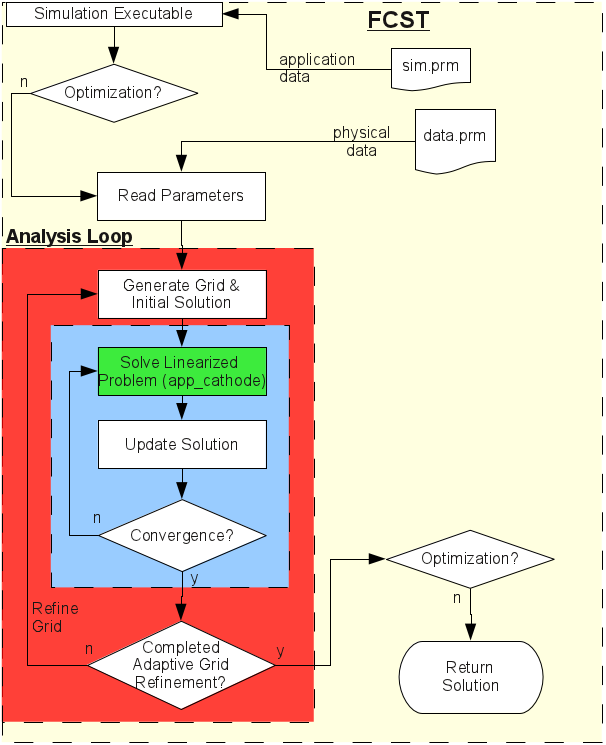
\includegraphics[width=0.5\textwidth]{figures/analysis_schematic.png}
\caption{Schematic of Fuel Cell Analysis Code.}
\label{analysis_schematic}
\end{center}
\end{figure}

In the next sections, first the OpenFCST graphical user interface is discussed. Then, the main and data files are discussed in detail. The files with extension .xml are read with the OpenFCST GUI. The files with extension .prm are ASCII files. The latter contain the same information, but they are easier to read in a text editor. OpenFCST can convert .prm files to .xml files easily. If you have a folder with a main.prm and a data.prm files (the data file name can be anything, but it must be specified in the main.prm file), then you can call OpenFCST as follows:
\begin{lstlisting}
$~/Openfcst/Install/bin/> ./fuel_cell-2d.bin -c main.prm
\end{lstlisting}
Then main and data files in XML format will be generated based on the main.prm file provided. The XML files can then be visualized and modified with the OpenFCST GUI.

%%==============
\section{OpenFCST examples}

The folder \texttt{examples} in the \texttt{Install} folder in OpenFCST contain an HTML manual with several examples. The examples are part of our testing suite to make sure that OpenFCST continues to provide the same results as new functionality is added. Each sub-directory in \texttt{examples} contains an explanation of the problem that is being solved as well as the data files to obtain the results. The easiest way to get started with OpenFCST is to run the example cases. We suggest that you do not modify the files in the examples folder, instead copy them to a different sub-folder such as \texttt{my\_data} so that you can still test your code with \texttt{run\_tests}.

The folder \texttt{examples/} contains .prm files. We recommend that you convert them to .xml files and then visualize them in the OpenFCST GUI. 

%%==============
\section{OpenFCST's graphical user interface}

%Purpose:
The OpenFCST graphical user interface (GUI) allows one to create, configure, and run simulations within a single application. All the OpenFCST simulation parameters are viewable and editable through the GUI. Using the GUI, one can browse through the hierarchy of parameters to edit numerous aspects of a simulation. Parameter descriptions are displayed by mousing over a parameter name. Once suitable simulation parameters have been selected, a simulation can be run from within the GUI. Simulation output such as text logging and a list of generated files are displayed within the GUI in a convenient manner.

One may create a new project, whereby default parameter files will be created in a step-by-step process. Alternatively, one can load an existing project. A project is made of two to three files:
\begin{itemize}
 \item \texttt{main.xml} contains the main selections for OpenFCST, such as the type of application, nonlinear solver, and type of study to be performed, i.e. one analysis run or a parametric analysis run.
 \item \texttt{data.xml} contains the parameters to setup the simulation for the selected application.
 \item \texttt{opt.xml} is an optional file used to setup parameters for optimization.
\end{itemize}
There files are discussed in more detail later in this guide.

Given the large number of parameters in a simulation, we recommend that new users start with a project from the \texttt{examples} directory since the step-by-step process requires an in-depth knowledge of the code. In order to generate a GUI project from the examples folder, go to an example folder such as \texttt{cathode/analysis}, and then generate the XML files from the parameter files using the OpenFCST:
\begin{lstlisting}
$~/Openfcst/Install/examples/cathode/analysis> fcst2D -c main.prm 
\end{lstlisting}

Using the \texttt{main.prm} file, the .xml files that constitute a project are generated. The following output will appear in the terminal:
\begin{lstlisting}
Parameters: main.prm
Creating converted main file in XML
YOU ARE CURRENTLY SOLVING A CATHODE MODEL
Application->DoF->BlockMatrix->OptimizationBlockMatrix
->FuelCellShop::Equation::NewFicksTransportEquation
->FuelCellShop::Equation::ElectronTransportEquation
->FuelCellShop::Equation::ProtonTransportEquation
->FuelCellShop::Equation::ReactionSourceTerms
->FuelCell::Application::AppCathode-2D
YOU ARE USING Newton3pp NEWTON SOLVER
Application->Copy->Newton3ppBase->->AdaptiveRefinement
Parameters: data.prm
Creating converted data file in XML
No opt file detected, skipping.
\end{lstlisting}
Then \texttt{main.xml} and \texttt{data.xml} files will be generated.
 
Once the files are generated, they can be loaded into the GUI.

%===============================
\subsection{Overview}

In order to start the OpenFCST GUI, go to the \texttt{/Install/bin} folder and run the executable \texttt{fcst\_gui}. The GUI will start by asking for the binary to be used to run the simulations. There are two possible files that can be used:
\begin{itemize}
 \item \texttt{fuel\_cell-2d.bin}
 \item \texttt{fuel\_cell-3d.bin}
\end{itemize}
Select the first executable to run two-dimensional simulations, e.g., cathode and MEA, and the second for three-dimensional simulations, e.g. \texttt{ohmic} application.

The main components of the GUI shown in Figure \ref{fig:GUI_overview} can be described as follows:
\definecolor{red}{RGB}{255,0,0}
\definecolor{pink}{RGB}{255,0,255}
\definecolor{yellow}{RGB}{200,255,0}
\definecolor{blue}{RGB}{0,0,255}
\definecolor{green}{RGB}{0,255,0}
\definecolor{grey}{RGB}{90,90,90}

\begin{itemize}
 \item \textbf{\textcolor{pink}{File menu:}} From this menu we can start a new project, open an existing project, save the current project, save a specific file from the current project, save the simulation log to a text file, and exit the GUI. 
 \item \textbf{\textcolor{red}{Parameter editing panel:} } This panel displays all the parameters of the loaded project. We can browse through the parameter hierarchy using the mouse to locate the parameter we desire. Descriptions/hints about a specific parameter are displayed by mousing over it.
 \item \textbf{\textcolor{yellow}{Start/next/end button:}} This button is used predominantly to progress our current project.
 \item \textbf{\textcolor{green}{Application Output:} } While running a simulation, text output describing the status of the simulation will be shown here.
 \item \textbf{\textcolor{blue}{Output Files:}} While running a simulation, OpenFCST will produce several output files. Clicking on any item displayed in this list will open the file with the operating system default program associated to the file's type. 
\end{itemize}

\begin{figure}[tbp]
\begin{center} 
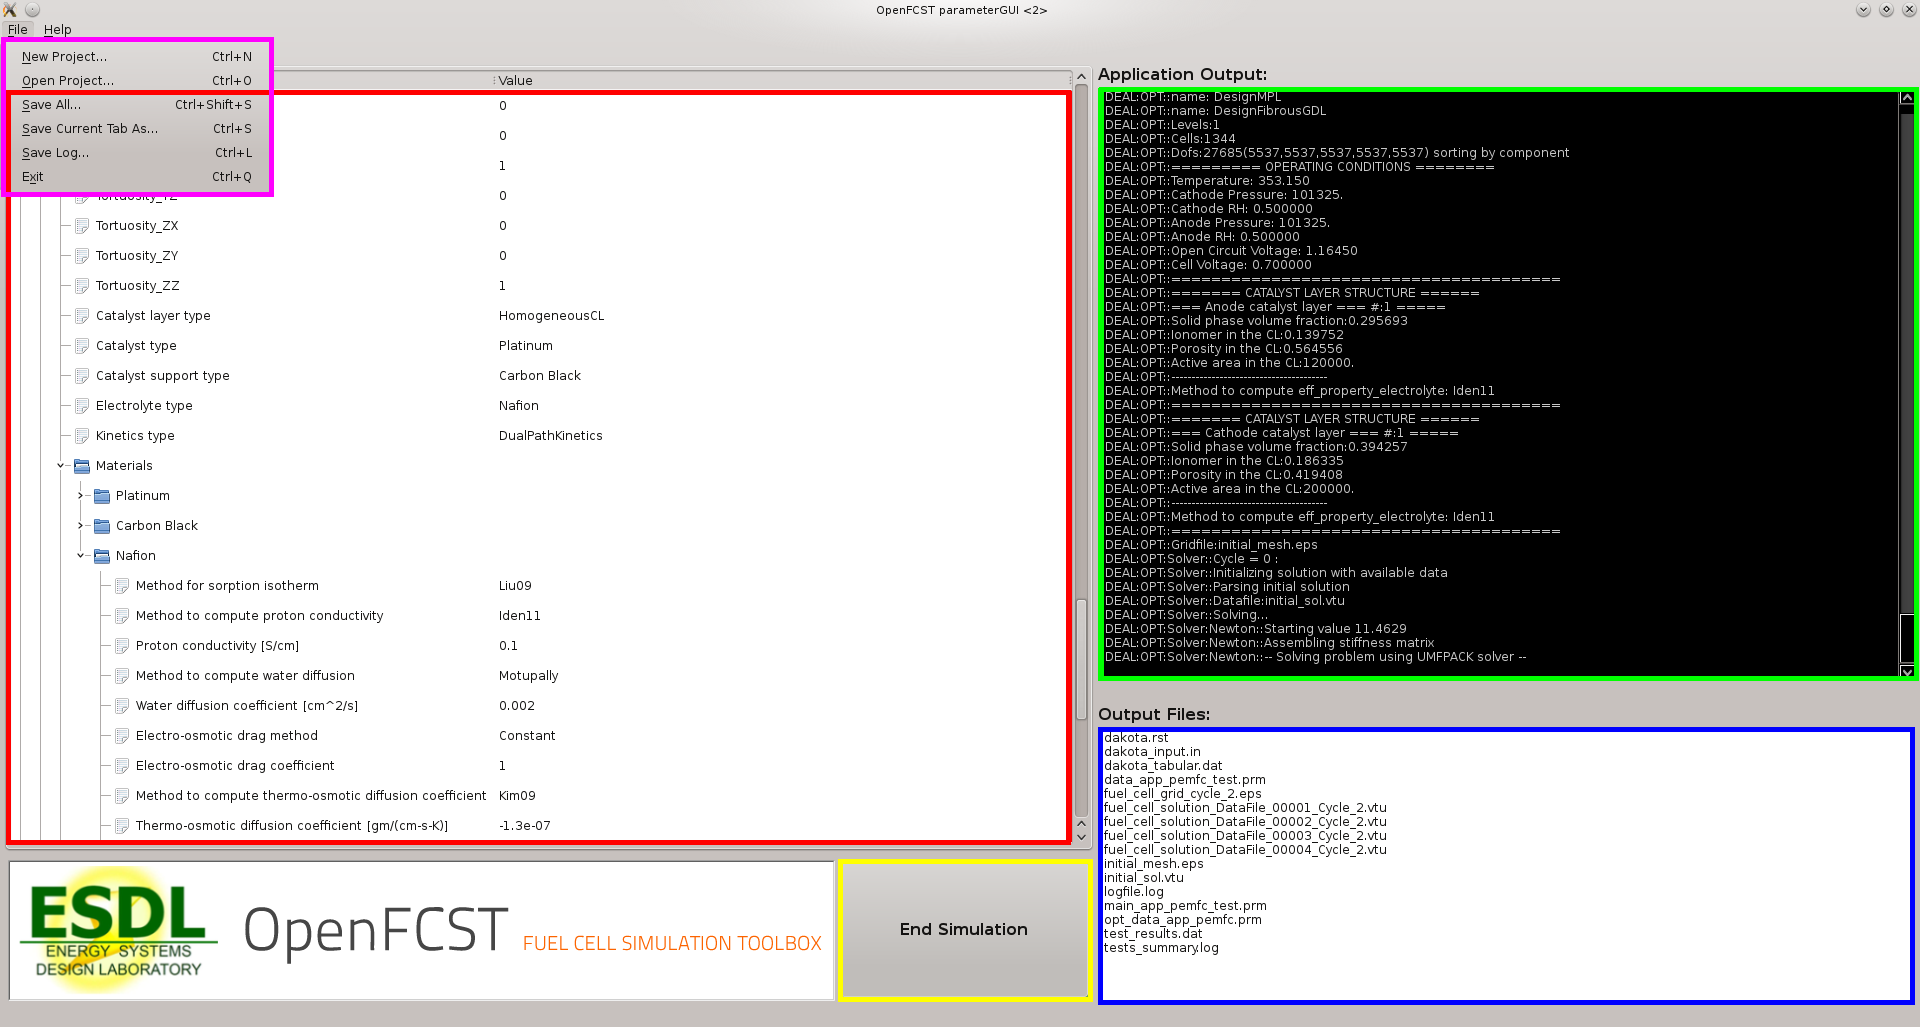
\includegraphics[width=\textwidth]{./figures/gui2.png}
\caption{Main window of the OpenFCST graphical user interface. Components of interest are highlighted.}
\label{fig:GUI_overview}
\end{center}
\end{figure}

%===============================
\subsection{How To's}
%---
\subsubsection{Start a New Project} \label{sec:start_new_project_gui}
\textcolor{red}{Warning:} Default parameter files created by OpenFCST version 0.2 require extensive modification in order to run a simulation. We suggest that users new to OpenFCST use the ``Open Project'' option explained later in this section.

Starting a new project from scratch using the GUI is simple:

\begin{enumerate}
 \item First, select the ``New Project'' option from the \textcolor{pink}{file menu}.
 \item A dialogue will open asking you to select a folder, i.e. a ``working directory''. This is the location  where your project file and simulation output will be placed. \textcolor{red}{Warning:} placing a project in a folder with an existing project may cause some files to be overwritten.
 \item Once a working directory has been selected, OpenFCST will generate a main parameter file. This file allows us to select important aspects of our simulation, such as the type of application we would like to run (Cathode simulation, non-isothermal application, etc) and the type of Newton solver we would like to use.
 \item At this point, clicking the \textcolor{yellow}{Next} button will instruct OpenFCST to read our main file and generate a corresponding data file. A data file includes important parameters pertaining to simulation aspects such as equations,  finite elements,  mesh refinement, and fuel cell material parameters. Additionally, an optimization file may be generated, depending on if you have compiled OpenFCST with Dakota.
 \item Now that we have edited our parameter files to our desire, clicking the \textcolor{yellow}{Run} button will start the simulation. Whilst the simulation is running, its status will be shown by the \textcolor{green}{Application Output panel} and a list of files generated by OpenFCST will be shown in the \textcolor{blue}{Output File panel}.
 \item If there are no errors, the simulation will run to completion.
\end{enumerate}

%---
\subsubsection{Open an Existing Project}\label{sec:open_existing_project_gui}
Opening an existing project using the GUI is a simple process, similar to starting a new one.

\begin{enumerate}
 \item Select ``Open Project'' from  the \textcolor{pink}{file menu}.
 \item You will be asked to specify the location of a \textbf{main} parameter file. \emph{Note:} The directory of the main file will be used as the project\textquoteright s working directory, i.e. the location where your project files and simulation output will be placed. 
 \item Once the location of the main file has been specified, you will be asked for the location of the \textbf{data} file.
 \item Once the location of the data file has been set, you can load additional files, such as optimization parameter files. It is not necessary to load these additional files. 
 \item Now you can edit the loaded files and run the simulation by clicking the \textcolor{yellow}{run} button, in the same fashion as described earlier in this section.
\end{enumerate}

%---
\subsection{Configuration}
The version of the OpenFCST binary you are using may have unique interface arguments. To maintain functionality between the GUI and the OpenFCST binary the following parameters are editable in the GUI's \textbf{settings.ini} file (which will be created in the same directory as the GUI once it is run). Typically,  these parameters do not need to be edited.

\begin{itemize}
 \item \textcolor{grey}{\textbf{OpenFCSTbin:}} The path to the OpenFCST binary you wish to use to run your simulations.
 \item \textcolor{grey}{\textbf{OpenFCSTparamArg:}} The command line argument which instructs OpenFCST to create a parameter file.
 \item \textcolor{grey}{\textbf{mainFileName:}} The name of the main file OpenFCST will create when generating a new Project.
 \item \textcolor{grey}{\textbf{dataFileName:}} The name of the data file which OpenFCST will create when generating a new Project.
 \item \textcolor{grey}{\textbf{optFileName:}} The name of the optimization file which OpenFCST will create when generating a new Project.
\end{itemize}

%---
\subsection{Reporting Errors}
In the case of program errors or crashes occurring,  please \htmladdnormallink{contact us}{http://www.esdlab.mece.ualberta.ca/contact.php}. 

Providing the following  will help us to resolve your issue:

\begin{itemize}
 \item a description of the circumstances in which the errors occurred and any error messages that you may have received;
 \item a copy of your parameter files (main.xml, data.xml, etc);
 \item the GUI log file (gui\_log.txt);
 \item simulation log files (which can be produced using the graphical user interface, and found in the project's working directory).
\end{itemize}

%%==============
%%==============
\section{The OpenFCST \texttt{main} file}

The \texttt{main} file is the initial file accessed by OpenFCST. The file contains two main subsections:
\begin{enumerate}
 \item \texttt{Simulator};
 \item \texttt{Logfile}.
\end{enumerate}

%-----
\subsection{\texttt{Simulator} section}
The \texttt{Simulator} section is used to setup the high-level parameters for the simulation such as the application to solve, the type of solver, and the type of results. This section is maybe the most important as it dictates the information that will appear in the data file for the GUI. Please note that some parameters cannot be modified once the data file has been generated. The parameters in this section are:
\begin{itemize}
 \item \texttt{simulator name}: This entry specifies the type of simulation that you would like to perform, e.g., solve a cathode model (\texttt{cathode}), a full MEA model (\texttt{MEA}), an electrical conduction problem (\texttt{ohmic}). The data file is dependent on the selection of this parameter, therefore, if the default data file is generated with one value, it will not work with others.
 \item \texttt{simulator specification}: This entry is only used with fluid flow applications to specify different sub-problems based on boundary conditions.
 \item \texttt{solver name}: This entry specifies if the problem is linear (Linear) or non-linear. For the latter, the OpenFCST team has implemented several Newton solvers that can be used. Note that the data file should be re-generated if the type of solver is changed.
 \item \texttt{solver method}: This entry can be used to add an additional loop during the solution stage after the analysis loop (see Figure~\ref{analysis_schematic}).
 \item \texttt{simulator parameter file name}: This entry should contain the name of the data file for the simulation. The data file should be in the same folder as the main file.
 \item \texttt{Analysis type}: This entry specifies if you would like to run a simulation for a specific cell operating condition, a polarization curve, a parametric study, or an optimization case. The options for each one of these cases are specified in the later subsections. For \texttt{Analysis}, no further information is required. For the other cases, the necessary information is specified next.
\end{itemize}

Subsections \texttt{Optimization}, \texttt{Parametric Study} and \texttt{Polarization Curve} are described next. For \texttt{Polarization Curve}, the following parameters can be specified:
\begin{itemize}
  \item \texttt{Polarization curve file output}: This entry specifies the file where the polarization curve results should be stored;
  \item \texttt{Initial voltage [V]}: Voltage at which the first point in the polarization curve will be evaluated;
  \item \texttt{Final voltage [V]}: Voltage at which the polarization curve will be terminated. Note that if the value is set, for example, to 0.6 V, then the polarization curve will not include this voltage (it will run down to 0.6~V plus increment);
  \item \texttt{Increment [V]}: Spacing between points in the polarization curve;
  \item \texttt{Adaptive Increment}: Set to true if you would like to reduce the voltage increment adaptively if convergence could not be achieved with the larger value;
  \item \texttt{Min. Increment [V]}: If Adaptive Increment is set to true, this value controls the minimum change in cell voltage before the polarization fails to converge and the voltage is updated again. Note that this value has to be positive as a value of zero would lead to an infinite loop.
\end{itemize}

Subsection \texttt{Parametric Study} is used when a parametric study is to be performed for a different variable than cell voltage. In this case, the most important parameter to specify is \texttt{Parameter name} which identifies the parameter that is to be modified. Any parameter in the OpenFCST data file can be modified following the format specified below. The parameters and how to modified are explained below:
\begin{itemize}
 \item \texttt{Parameter file output}: File where the parametric study results should be stored.
 \item \texttt{Parameter name}: Enter the name of the parameter you would like to study. Use one of the following formats:
 \begin{itemize}
   \item For normal parameter: \texttt{Subsection\_1$>>$Subsection\_2$>>$Value};
   \item For boundary value or graded: \texttt{Subsection\_1$>>$Subsection\_2$>>$Material\_id:Value},
 \end{itemize}
   where \texttt{Subsection\_1} and \texttt{Subsection\_2} would be the sections where the parameter is found in the data file. For example, if we would like to change the temperature of the cell, we would write \texttt{Fuel cell data$>>$Operating conditions$>>$Temperature cell}.
   \item \texttt{Initial value}: Enter the value you would like to start the parametric study from.
   \item \texttt{Final value}: Enter the final value for the parametric study.
   \item \texttt{Increment}: Spacing between points in the parametric study.
   \item \texttt{Adaptive Increment}: Set to true if you would like to reduce the increment adaptively if convergence could not be achieved with the larger value
   \item \texttt{Min. Increment}: If Adaptive Increment is set to true, this value controls the minimum change in parameter before the polarization fails to converge and the voltage is updated. Note that this value has to be positive as a value of zero would lead to an infinite loop.
   \item \texttt{Parameter values}: If you would like to run the parametric study for only some points, then a list containing the discrete values of a parameter of study can be included here. If this value is empty, then the Initial and Final value entries are used, if this list is filled, then the list is used instead.
\end{itemize}

Subsection \texttt{Optimization} is used when an optimization study is to be performed. In this case, the file that includes all optimization parameters is to be included here. There are only two entries in this subsection:
\begin{itemize}
 \item \texttt{optimization parameter file name}: Enter here the name of the optimization file. By default, if using the GUI, opt.xml should be used.
 \item \texttt{Dakota direct}: Set to true if you would like OpenFCST to directly interact with Dakota, i.e. OpenFCST will call Dakota as needed to run the optimization simulation. If set to false, then OpenFCST will run once and output a file that Dakota can read. In this case Dakota would be the optimization driver.
\end{itemize}

\subsection{The \texttt{Logfile} section}
The \texttt{Logfile} section is used to specify where the output from OpenFCST should be stored and how much output should be stored.

%%==============
\section{The OpenFCST \texttt{data} file}

The OpenFCST data file will change depending on the parameters that are specified in the main file, but in general it contains the following sections:
\begin{itemize}
 \item \texttt{Adaptive refinement}: This section is used to control adaptive refinement options. Only advanced users should modify this section.
 \item \texttt{Newton}: Section used to specify the parameters that control the Newton solver to solve the problem.
 \item \texttt{Grid generation}: Section used to specify the geometry of the domain. \textbf{This section is critical} as the ID specified in this section for \texttt{material\_ID} and \texttt{boundary\_ID} are used to impose the appropriate initial and boundary solution in section Equations. 
 \item \texttt{Discretization}: This section is used to specify the type of finite element used to discretize the governing equations. The quadrature formula and degree are also set here.
 \item \texttt{System management}: This section is used to specify the equations that need to be solved. In most cases, this section is filled automatically by the application.
 \item \texttt{Equations}: \textbf{This section is critical}. In this section, the initial solution and boundary conditions for each equation need to be specified. The values are specified using the following format \texttt{material\_ID}:value and \texttt{boundary\_ID}:value. This section will be discussed below in more detail.
 \item \texttt{Reaction source terms}: This section is used to turn on/off source terms for the equations.
 \item \texttt{Initial Solution}: This section is used to control initialization and output of the initial solution. OpenFCST can generate a default initial solution or a previous solution can be used as an initial guess. This section allows users to create an initial solution for later use and to load previous solutions as an initial solution. Note that the initial and final solution have to be on the same mesh. OpenFCST also allows users to output the initial solution here.
 \item \texttt{Linear Solver}: This section is used to select the linear solver that users want to use. Several direct and iterative solvers are available. For non-linear problems, only direct solvers, e.g., \texttt{UMFPACK} and \texttt{MUMPS}, and iterative solver ILU-GMRES are satisfactory due to the nature of the Jacobian matrix to be inverted. 
 \item \texttt{Fuel cell data}: This is the most important section of OpenFCST for a user as it encapsulates all the fuel cell information, e.g., operating conditions, type of kinetic model, catalyst layer model and GDL type.
 \item \texttt{Output}: This subsection is used to specify the output format for the mesh and the output solution data. In general, we recommend EPS and VTU formats for grid and data respectively. Only advanced users should modify this section.
 \item \texttt{Output Variables}: This section is used to request OpenFCST to calculate and output a variety of functionals, i.e., integral quantities, at postprocessing such as current density and water crossover.
 \item \texttt{Postprocessing}: This section is used in order to provide additional information to compute the functionals specified in \texttt{Output Variables}.
\end{itemize}

%---
\subsection{The \texttt{Adaptive refinement} section}

This section is used in combination with the flags in \texttt{Grid generation} section to control refinement levels and output options for the mesh and solution. 

This section has the following entries:
\begin{itemize}
 \item \texttt{Number of Refinements}: This parameter is used to define the number of times the mesh will be refined. The minimum value is one, i.e., only the original mesh is solved. At each adaptive refinement level, either all the cells (global) or 30\% of the cells with largest error (computed using an error estimator; adaptive) are split into four. The process is repeated at each refinement level. An example of mesh that is refined globally several times and an adaptively refined mesh is shown in Figure \ref{fig:grid_adaptive_refinement}.
   \item  \texttt{Refinement}: This flag specifies the type of refinement to be used if in \texttt{Adaptive refinement} section you decided to solve the problem in several meshes. Mainly two options are available:
  \begin{enumerate}
   \item global: At each refinement level, each cell in the domain is divided into four new cells.
   \item adaptive: At each refinement level, a percentage, specified in texttt{Refinement threshold}, of cells with the largest error are divided into four cells. Also, the percentage of cells in \texttt{Coarsening threshold} with the smallest error are re-merged into one cell if they had been previously refined. 
  \end{enumerate}
 \item \texttt{Refinement threshold}: For adaptive refinement, the percentage of cells with largest error that should be refined.
 \item \texttt{Coarsening threshold}: For adaptive refinement, the percentage of cells with smallest error that should be coarsened.
 \item \texttt{Output initial mesh}: Set flag to true if you want to output an EPS figure of the initial mesh using the value in \texttt{Output initial mesh filename}.
 \item \texttt{Output initial mesh filename}: Filename of where the initial mesh will be output.
 \item \texttt{Output intermediate solutions}: Set flag to true if you would like the solution at each grid refinement to be output. Please note that outputting the solution is time consuming.
 \item \texttt{Output intermediate responses}: Compute the functionals in \texttt{Output variables} at each grid refinement. Use this option if you want to perform a grid refinement study. Please note however that computing the functionals is time consuming.
 \item \texttt{Output final solution}: Output the final solution to a file.
 \item \texttt{Compute errors and convergence rates}: Internal option for developers. Always set this value to false.
 \item \texttt{Use nonlinear solver for linear problem}: Internal option for developers. Always set this value to false.
\end{itemize}

\begin{figure}[tbp]
\centering
\minipage{0.2\textwidth}
  
\includegraphics[width=\linewidth]{figures/grid_no_refinement.png}
  \caption{Initial Grid.}
\endminipage\hfill
\minipage{0.2\textwidth}
  
\includegraphics[width=\linewidth]{figures/grid_first_refinement.png}
  \caption{Global $1^{st}$ Refinement.}
\endminipage\hfill
\minipage{0.2\textwidth}
  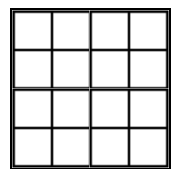
\includegraphics[width=\linewidth]{figures/grid_second_refinement.png}
  \caption{Global $2^{nd}$ Refinement.}
\endminipage\hfill
\minipage{0.2\textwidth}
  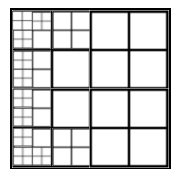
\includegraphics[width=\linewidth]{figures/grid_adaptive_refinement.png}
  \caption{Adaptive Refinement.}
  \label{fig:grid_adaptive_refinement}
\endminipage\hfill
\end{figure}


In order to control the type of refinement, \texttt{Grid generation>>Refinement} is used. This value can be set to adaptive or global in order to specify the type of refinement. Furthermore, if adaptive is used, the percentage of cells that are refined and coarsened is given by \texttt{Grid generation>>Refinement threshold} and \texttt{Grid generation>>Coarsening threshold}.

%---
%---
\subsection{The \texttt{Newton} section}

This section specifies the parameters that are used to control the Newton iteration for the case of non-linear problems. There are many parameters most of which are self-explanatory. The most critical parameters are:
\begin{itemize}
 \item \texttt{Max steps}: Used to limit the number of iterations carried out by the Newton solver.
 \item \texttt{Tolerance}: The value of the L${}^2$-norm of the residual. Ideally, this tolerance should be kept at $1.0e^{-9}$. However, in certain circumstances, convergence with that tolerance may not be possible or feasible given the computational time. In these scenarios it is possible to reduce the tolerance to $1.0e^{-4} - 1.0e^{-6}$ while still keeping reasonable accuracy.
 \item \texttt{Reduction}: Use if you want convergence to be accomplished after the initial residual (or whatever criterion was chosen by the solver class) is reduced by a given factor. This is useful in cases where you don't want to solve exactly, but rather want to reduce the residual by a small amount. We recommend setting this value always to $1.0e^{-20}$.
\end{itemize}

In order to control the solution output during the Newton iteration, the following four parameters can be used
\begin{itemize}
 \item \texttt{Debug level}: Write debug output to the logfile. The higher the number, the more output. The range is between 0 and 3.
 \item \texttt{Debug residual}: Output the residual at every Newton iteration. This then can be used to locate errors/bugs in the code.
 \item \texttt{Debug solution}: Output the solution at every Newton iteration. This then can be used to locate errors/bugs in the code.
 \item \texttt{Debug update}: Output the solution update at every Newton iteration. This then can be used to locate errors/bugs in the code.
\end{itemize}

The parameters \texttt{special\_block\_i} are internal variables. They should not be used by the users.

%---
%---
\subsection{The \texttt{Grid generation} section}

The \texttt{Grid generation} section is one of the most important sections in OpenFCST, together with the \texttt{Fuel cell data} section. This section is used to define the geometry for the fuel cell. The fuel cell geometry is represented by the following data:
\begin{itemize}
 \item Length of each fuel cell layer, channel, and land.
 \item A collection of \texttt{Material ID}s used to identify each layer in the domain to the layers in the \texttt{Fuel cell data} section.
 \item A collection of \texttt{Boundary ID}s used to identify the boundaries of the domain where boundary conditions are applied.
\end{itemize}
These sections are key and are used in the \texttt{Equations} section to specify initial solution and boundary conditions and in \texttt{Fuel cell data} to associate each layer in the geometrical domain with the corresponding fuel cell properties.

The \texttt{Grid generation} section contains many entries. The following entries are used to specify the type of mesh and if any refinement on the mesh should be performed prior to the simulation:
\begin{itemize}
 \item \texttt{Type of mesh}: This entry specifies the type of mesh you would like to generate. You have two main options \texttt{ExternalMesh} will load an external mesh for your simulation. The other options use OpenFCST internal mesh generator to directly generate the geometry. 
 \item \texttt{File name}: If type of mesh has been set to \texttt{ExternalMesh}, this section should contain the name of the mesh file you would like to load. The file should be in the same folder as main.
 \item \texttt{File type}: Specify the extension of the file.
 \item \texttt{Initial refinement}: Number of times we want to globally refine the original grid before starting to solve.        
\end{itemize}

The following option is used to specify the numbering scheme for the degrees of freedom in the mesh. By default, degrees of freedom (DoFs) are sorted by component, but the following flag can be used to sort the DoFs using other schemes
\begin{itemize}
 \item \texttt{Sort Cuthill-McKee}: Organize the degree of freedom numbering for the mesh using the Cuthill-McKee algorithm.
\end{itemize}

The subsection \texttt{Internal mesh generator parameters} is only needed if the OpenFCST internal mesh generator is used. If it is not used, the section can be almost entirely ignored since the \texttt{ExternalMesh} should already contain material and boundary IDs. Some post-processing routines however might use several entries such as \texttt{Cathode CL thickness [cm]} and \texttt{boundary IDs}, so it might be necessary to fill out these values even if using an \texttt{ExternalMesh} in some instances.

The Dimensions subsection in \texttt{Internal mesh generator parameters} is used to specify the dimensions of each parameter in the cell. It contains the following:
\begin{itemize}
  \item \texttt{Cathode current collector width [cm]}: Thickness of the ribs of the bipolar plates (BPP) [cm].
  \item \texttt{Cathode channel width [cm]}: Thickness of the channels on the BPP [cm].
  \item \texttt{Cathode CL thickness [cm]}: Thickness of the cathode catalyst layer [cm].
  \item \texttt{Cathode GDL thickness [cm]}: Thickness of the cathode gas diffusion layer [cm].
  \item \texttt{Cathode MPL thickness [cm]}: Thickness of the cathode microporous layer [cm].
  \item For the remaining entries, please mouse over the entry in the GUI for meaning.
\end{itemize}

Subsection \texttt{Mesh refinement parameters}:
\begin{itemize}
  \item \texttt{Initial vertical cell count}: Number of cells we want in the y-direction of the original grid before starting to solve
  \item \texttt{Horizontal division of cathode GDL}: Number of cells we want in x-direction in the cathode GDL layer
  \item \texttt{Horizontal division of cathode CL}: Number of cells we want horizontally in the cathode CL layer
  \item For the remaining entries, please hover the mouse over the entry in the GUI for its meaning.
\end{itemize}

Subsection \texttt{Material ID} is used to define the material ID for each component of the cell. The material ID is used in \texttt{Fuel cell data} to associate each one of the cells in the mesh with the desired fuel cell properties. The entries in this section look as follows:
\begin{itemize}
  \item \texttt{Test}: Material ID for GridTest.
  \item \texttt{Cathode current collector}: Current collector material\_id.
  \item \texttt{Cathode gas channel}: Cathode gas channel material\_id.
  \item \texttt{Cathode GDL}: Cathode gas diffusion layer material\_id.
  \item \texttt{Cathode MPL}: Cathode microporous layer material\_id.
  \item For the remaining entries, please hover the mouse over the entry in the GUI for its meaning.
\end{itemize}

Subsection \texttt{Boundary ID} is used to define the boundary ID for each boundary in a fuel cell. These IDs are used in Equations section to specify Dirichlet and Neumann boundary conditions for each equation at each one of the defined boundaries. \textbf{The number 255 defines an interior boundary condition in deal.II. All internal boundaries MUST have a 255 boundary ID.} The entries in this section appear as follows:
\begin{itemize}             
  \item \texttt{c\_Ch/GDL}: Cathode gas channel and gas diffusion layer boundary\_id. 
  \item \texttt{c\_BPP/GDL}: Cathode bipolar plates and gas diffusion layer boundary\_id.
  \item \texttt{c\_GDL/CL}: Cathode gas diffusion layer and catalyst layer boundary\_id. Since this boundary is an internal boundary in most cases, it must be set to 255.
  \item For the remaining entries, please mouse over the entry in the GUI for meaning.
\end{itemize}

%--------------------
\subsection{The \texttt{Discretization} section}

The \texttt{Discretization} section is used to select the finite element discretization and the quadrature formula used to evaluate the weak form integrals. The key parameters defined in the subsection are:
\begin{enumerate}
\item \texttt{Element}: Defines the finite element discretization for each equation. This parameter is discussed in detail below.
\item \texttt{Degree Mapping}: Defines the geometric mapping. In most cases a linear mapping is used, i.e. set the value to 1.
\item \texttt{Boundary fluxes}: Set to true if there are any either Neumann or Robin boundary conditions. If the parameter is set to false, then OpenFCST will skip looping over boundaries resulting in faster computational speeds.
\item \texttt{Interior fluxes}: Set to true if there are any flux jumps between elements. This will only occur if using a Discontinuous Galerkin (DG) formulation. So far we have not implemented any DG schemes in OpenFCST.
\item \texttt{Matrix}: Used to control the number of quadrature points required to evaluate the integrals on the left hand side of the local weak form defining the partial differential equation. 
\item \texttt{Residual}: Used to control the number of quadrature points required to evaluate the integrals on the right hand side of the local weak form defining the partial differential equation. 
\end{enumerate}

Of the above parameters, \texttt{Element} is of critical importance as it specifies the type of finite element used for the spatial discretization. If only one equation is used, the element is specified as:
\begin{lstlisting}
  set Element = FE_Q(2)
\end{lstlisting}
where $FE\_Q(2)$ refers to the type of element, i.e. Lagrange element ($FE\_Q$), and the number in parenthesis, i.e, 2, is the order of the element, in this case quadratic. 

For system of equations, the finite element discretization for each equation needs to be specified. For example, for a system of five equations we would write
\begin{lstlisting}
  set Element = FESystem[FE_Q(2)^5] 
\end{lstlisting}
where FE\_Q(2) refers to the type of element and the number five in FE\_Q(2)\string^5 refers to the number of variables included in the quadratic category. If we want to use different elements for different variables we would specify it by separating the elements with a dash. For example, if we wanted the first two elements solved with a cubic Lagrange element and the last three solved with a linear Lagrange element approximation, we would insert the following line. FESystem[FE\_Q(3)\string^2-FE\_Q(1)\string^3]

The final two sections in \texttt{Discretization}, are
\begin{enumerate}
\item \texttt{Matrix};
\item \texttt{Residual}.
\end{enumerate}
Matrix and Residual control the number of quadrature points required to evaluate the integrals in the local weak form of our partial differential equation. The default value of -1 will set the number of quadrature points to the order of the finite element used plus one in each direction, e.g., for second order elements, number of quadrature points in each direction is $2 + 1 = 3$ (in 2D, using quadratic elements, the number of quadrature points would be 9). Assigning a default value of $-1$, for most cases, should be sufficient to achieve an exact solution of the integrals.

%--------------------
\subsection{The \texttt{System management} section}

The \texttt{System management} subsection is responsible for defining the \texttt{Solution variables} \&  \texttt{Equations} being used. This section is populated by the application directly and should not be modified by the users.

%--------------------
\subsection{The \texttt{Equations} section}

This section is responsible for specifying the initial solution and boundary conditions for the application at hand. The section is subdivided in one subsection per equation that needs to be solved. Inside each subsection, the main section needs to be specified:
\begin{itemize}
 \item \texttt{Initial data}: It is used to specify a piece-wise initial solution for the simulation. It contains two main entries:
 \begin{itemize}
  \item \texttt{Variable initial data}: If set to true and the application has implemented a variable initial guess, the variable initial guess is used.
  \item \texttt{variable\_name}: The name of this section corresponds to the variable we are trying to initialize. In this section, for each material ID a value needs to be given in order to setup an initial solution. The initial solution might be overwritten using the section \texttt{Fuel cell data>>Operating conditions}, however the map of material ID must be included here. If you have a mesh with two material IDs, e.g. CL is 5 and GDL is 8, and you would like to setup the initial solution for your variable to 0.2 and 0.3 in CL and GDL respectively, then the entry will be: \texttt{5:0.2, 8:0.3}. For each solution variable we have a comma-separated list of material ID, colon, value. 
 \end{itemize}
 \item \texttt{Boundary conditions}: Provides the ID for the type of boundary condition that you would like to have.
 \item \texttt{Boundary data}: Provides the value for Dirichlet, Neumann and Robin boundary conditions. As for the case of \texttt{Initial data}, the same format is used. Again this section is mandatory and it is the user's responsibility to create the appropriate map.
\end{itemize}

%--------------------
\subsection{The \texttt{Reaction source terms} section}
This section is used to turn on/off source terms for the equations.

%--------------------
\subsection{The \texttt{Initial Solution} section}

This section is used to control the initial guess that the user would like to use. As specified in \texttt{Equations}, a piece-wise approximation can be used as an initial guess. Another possibility is to use a previous solution as an initial guess. In this case, simulation is run first with the `\texttt{Output solution for transfer}' option set to true. This will produce a hidden file containing the solution. This solution can then be read in if `\texttt{Read in initial solution from file}' is set to true and the new boundary conditions are applied. Reading in an old solution might be beneficial when convergence becomes an issue if the initial solution is similar to the new solution you are trying to obtain, i.e. all parameters are the same but one, e.g. when running a polarization curve. 

Two more parameters appear in this section:
\begin{itemize}
 \item \texttt{Output initial solution}: This option is usually used for debugging purposes for developers in order to make sure the initial solution is specified correctly.
 \item \texttt{Initial solution output file}: Specifies the name of the output file where the initial solution will be stored if the flag above is set to true.
 \item \texttt{Use pre-defined initial solution}: Some applications, like MEA, have a pre-defined initial solution. If set to true, this pre-defined solution is used.
\end{itemize}

%--------------------
\subsection{The \texttt{Linear Solver} section}
 
In this section, the linear solver to be used for solving the problem, either the full problem or the linearized equations in the case of a non-linear system, is specified. The most important parameter to select here is the \texttt{Type of linear solver} parameter. The parameter \texttt{Assemble numerically} is set to true if you would like to evaluate the Jacobian for the Newton loop numerically. This is extremely time consuming and therefore should only be used if an analytical Jacobian is not developed. All applications in OpenFCST use an analytical Jacobian. The other parameters are used to control the convergence of the program similar to the Newton section.
 
%--------------------
\subsection{The \texttt{Fuel cell data} section}

\texttt{Fuel cell data} subsection is the most important section in OpenFCST project as it specifies all relevant properties pertaining to operating conditions and each respective layer in a fuel cell. The section is divided into the following main subsections:  
\begin{enumerate}
  \item \texttt{Operating conditions}: Specify operating conditions for the fuel cell. It contains the following entries:
  \begin{itemize}
   \item \texttt{Adjust initial solution and boundary conditions}: Use the parameters in Operating conditions to create an initial solution and overwrite the boundary conditions for the problem specified in \texttt{Equations>>Initial Data} using the parameters in this section. This is the recommended option as it will directly calculate the appropriate relative humidity for your cell.
   \item \texttt{Temperature cell}: Fuel cell temperature in Kelvin.
   \item \texttt{Cathode pressure}: Cathode pressure in Pascals.
   \item \texttt{Cathode initial oxygen mole fraction (prior to humidification)}: Oxygen molar fraction prior to humidification. For example, 0.21 for air.
   \item \texttt{Cathode relative humidity}: Relative humidity as a fraction, i.e., between 0 and 1.
   \item All other parameters are entered using the same units. Their meaning is self-explanatory from the GUI.
  \end{itemize}
  \item \texttt{Materials}: This section includes the properties of gases and other materials that are used in multiple layers.
  \item Subsections defining every layer needed for the given application.
\end{enumerate} 

For each layer in a fuel cell, a subsection is defined here. All layers have the following common entries:
\begin{itemize}
 \item \texttt{Material id}: This integer number should be set to the material ID in the computational mesh that corresponds to the layer you would like to use the properties in this section for. If this section is a catalyst layer, then the material ID number corresponds to the number used in \texttt{Grid generation>>Internal mesh generator parameters>>Material ID>>Cathode CL}. \textbf{This entry is extremely important.}
 \item \texttt{PSD parameters}: This subsection is used to specify a pore-sized distribution for the layer. This section is not used in release 0.2.
 \item \texttt{Generic data}: This subsection is used to specify porosity, permeability and other properties that relate to a porous layer.
 \item \texttt{Layer type}: This drop down menu is very important as it specifies the layers that are currently available in the OpenFCST library. The value used here corresponds to a sub-section below if any parameters are needed from file. Only the properties in that sub-section (if defined) are needed to specify your layer. Currently only a few layer types are available: a dummy layer where all parameters can be specified, a design layer where parameters are obtained using effective medium theory as in reference \cite{Secanell07b}, and a limited number of commercial layers. \textbf{Input from users is needed to improve this database.}
\end{itemize}
Other entries are specific to each layer. They are self-explanatory by mousing over the parameters in the GUI. Here we will discuss the parameters in subsection \texttt{Cathode catalyst layer} in detail as it is the most complex entry. In this subsection we have the following additional entries
\begin{itemize}
 \item \texttt{Catalyst type}: Drop-down menu in order to select the appropriate catalyst from the OpenFCST database.
 \item \texttt{Catalyst support type}: Drop-down menu in order to select the appropriate catalyst support from the OpenFCST database.
 \item \texttt{Electrolyte type}: Drop-down menu in order to select the appropriate electrolyte from the OpenFCST database.
 \item \texttt{Kinetics type}: Drop-down menu in order to select the appropriate kinetics from the OpenFCST database.
\end{itemize}
For each one of the types in the drop-down menu either all properties are specified in OpenFCST, or several parameters are required from the user. In the latter case, a sub-folder is available to modify the parameters. For catalyst, catalyst support, and electrolyte, the properties of the materials are in sub-folder \texttt{Materials}. For the case of the kinetics, the folder \texttt{Kinetics} contains the sub-folders for the different options. As in the case of the layer, only the relevant sub-section with the name of the type selected is applicable and can be modified.

The OpenFCST team has implemented several multi-step kinetic models discussed in references \cite{Secanell08}, \cite{Moore13} and \cite{Secanell14}. In particular, the \texttt{DualPathKinetics} model is used for the hydrogen oxidation reaction and the \texttt{DoubleTrapKinetic} model is used for the oxygen reduction reaction. These models can be used with any of the applications here.

There are a large number of parameters in each subsection. Each parameter name is either self-explanatory or an explanation is shown by hovering the mouse over the parameter. If further information is needed, the users can go to the class documentation where additional information regarding each parameter is available.

%--------------------
\subsection{The \texttt{Output} section}
This subsection is used to specify the output format for the mesh and the output solution data. In general, we recommend EPS and VTU formats for grid and data respectively. Only advanced users should modify this section.

%--------------------
\subsection{The \texttt{Output Variables} section}
In this section, it is possible to specify integral equations that you would like to evaluate after the solution has been obtained such as current density, water crossover, and others. 

%--------------------
\subsection{The \texttt{Postprocessing} section}
This section is used to input information to some \texttt{Output Variables} that might require it.

% 
% 
% \subsection{Parameter/Optimization Application File}
% 
% 
% \item
% \texttt{opt\_app\_parametric\_default.prm}
% 
% The \texttt{opt\_app\_parametric\_default.prm} is used when carrying out parametric studies.
% 
% 
% 
% \begin{lstlisting}
% ######################################################################
% #
% #  This file is used to run a multi-dimensional parametric study. 
% #  See end of file for list of possible design variables.
% #
% ######################################################################
% 
% subsection Optimization Parameters
%   
% #### NOTE THAT THIS SECTION ONLY EXISTS WHEN RUNNING IN OPTIMIZATION MODE ###
% ####----------------------------------------------------------------------###
%     subsection Optimization Program Options
%       set Use dakota input file = false				# (default) false
%       set Dakota_Input_File = dakota_input.in			# not needed if -Use dakota input file = false-	
% 
%       set Optimization method = multidim_parameter_study 	# multidim_parameter_study | optpp_q_newton | nl2sol | ncsu_direct
%     end
% 
%     subsection Design Variables
%       set num_design_variables = 1			# 2
%       set DV_0_name = V_cell  					# P_cell 
%       set DV_1_name = T_cell						# P_c 	| RH_a
%       set DV_2_name = prc_Pt_c					# RH_c 	| prc_Pt_c
% 
%       #######	  Lower Bound 	 		 #######
%       ####### lb < -1e30 for -inf #######
%       #---------------------------------#
% 	set DV_0_lb = -1.1			# V # Changed to -1.1, force dekota to start at -1.1
% 	set DV_1_lb = 303				# K #  
% 	set DV_2_lb = 0.2				# % # 
% 
%       #######	 Upper Bound 			#######
%       ####### ub > 1e30 for inf #######
%       #-------------------------------#
% 	set DV_0_ub = -0.1			# V # 
% 	set DV_1_ub = 353				# K # 
% 	set DV_2_ub = 0.5				# % #
% 
%       ####### 						Parameter Study Partitions						  #######
%       ### NOTE: Evaluated at n+1 points between lower and upper bound ###
%       ###-------------------------------------------------------------###
% 	set DV_0_partition = 50
% 	set DV_1_partition = 8
% 	set DV_2_partition = 10
%       end
% 
% 	subsection Responses
% 	  set num_objectives = 1
% 	  set num_nl_constraints = 0 			# (default) 0
% 	  set num_eq_constraints = 0			# (default) 0
% 
% 	  set RESP_0_name = current
%       end
%   end
% \end{lstlisting}
% 
% 
% 
% 
% Located at the bottom of all \texttt{opt\_app} files in both parametric \& optimization is a list of design variables available for the user to carry out a parametric studies or optimization. As of \textbf{1-SEP-2013} the following table lists the current parameters that can be passed to DAKOTA for parametric studies/ optimization.
% 
% If the user requires additional variables for parametric/optimization studies, modification of the \\ \texttt{dakota\_application.cc} file should be carried out. 
% 
% \bigskip
% 
% \begin{lstlisting}
%       ######### List of Possible Design Variable Names #########
%       #########----------------------------------------#########
% #	//		Conventional_CL.cc
% #	V_Pt_c | V_Pt_a		// Platinum loading per unit volume [mg/cm3] 	(Cathode | Anode)
% #	prc_Pt_c | prc_Pt_a			// Platinum loading on support [%wt] 		(Cathode | Anode)
% #	prc_N_c | prc_N_a				// Electrolyte loading [%wt] 			(Cathode | Anode)
% #	Av_c | Av_a							// Active area [cm^2/cm^3] 			(Cathode | Anode)
% 
% #	//		Agglomerate_CL.cc
% #	r_agg_c	| r_agg_a			// Radius of the agglomerate [nm] 		(Cathode | Anode)
% #	r_agg								// Radius of the agglomerate [nm] **possibly redundant**
% #	epsilon_agg_c | epsilon_agg_a		// Agglomerate porosity 			(Cathode | Anode)
% #	epsilon_agg									// Agglomerate porosity **possibly redundant**
% 
% #	//		Operating_Conditions.cc
% #	V_cell					// Cell Voltage
% #	T_cell					// Cell Temperature  
% #	dV_a						// Voltage drop in the Anode
% #	P_c | P_a				// Pressure  					(Cathode | Anode)
% #	
% #	RH_c | RH_a				// Relative Humidity 				(Cathode | Anode) 
% #	OCV								// Open Circuit Voltage
% 
% #	//		Geometries.cc 
% #	L_CCL | L_ACL					// CL thickness  				(Cathode | Anode)
% #	L_CGDL | L_AGDL				// GDL thickness 				(Cathode | Anode)
% #	L_CMPL | L_AMPL				// MPL thickness 				(Cathode | Anode) 
% #	Ch_width							// Channel Width 				(Cathode | Anode)
% 
% \end{lstlisting}
% 
% 
% 
% \paragraph{Optimization Program Options:}
% 
% The \texttt{Optimization Program Options} of the \texttt{opt\_app} parametric file is responsible for telling OpenFCST whether it is required to formulate its own \texttt{dakota\_input.in} file or if you are supplying DAKOTA with a predefined input file (\textit{line 13 \& 14}). 
% 
% 
% \paragraph{``Use dakota input file'' \& ``Dakota\_Input\_File'':}
% 
% If \texttt{Use dakota input file} is set to \texttt{false} then OpenFCST will pass on the information specified in the \texttt{opt\_app\_parametric\_default.prm} file and DAKOTA will print out a new \texttt{dakota\_input.in} at run time. If however it is set to \texttt{true} we are telling OpenFCST that we have already specified an input file and that DAKOTA should use this directly rather than reading the information from the rest of the \texttt{opt\_app} file.
% 
% \paragraph{Note:} 
% 
% For completeness \texttt{``Use dakota input file'' \& ``Dakota\_Input\_File''} have been included in the default parametric file, however, when the user is not using their own \texttt{dakota\_input.in} file both line 13 \& 14 can be deleted.
% 
% Given that in most cases the user specifies all the parametric \& optimization information in the \texttt{opt\_app} file. The following descriptions will be relevant for cases when \texttt{Use dakota input file = false}.
% 
% \paragraph{Optimization Method:}
% 
% The \texttt{Optimization method} command is used to specify the type of study that is being carried out (optimization, parametric study, least squares fit, ...) for additional information on \texttt{Optimization methods} see section \ref{Optimization_using_FCST}. In our case we are looking to carry out a parametric study so the \texttt{multidim\_parameter\_study} should be specified.
% 
% \paragraph{Design Variables:}
% In the design variables section (\textit{line 19-45}) we specify the number of design variables that we want to change (\textit{line 20}), the upper and lower bounds for that variable (\textit{line 25-37}), and the number of points that we want to evaluate between the upper and lower bounds (\textit{line 39-45}).
% 
% 
% \paragraph{num\_design\_variables:}
% In the example above we have specified one design variable \texttt{V\_cell} for a  single parametric study. The corresponding upper, lower bounds, and partitions can be found at line 28, 35, and 42.
% 
% If the user wants to conduct a multi-dimensional parametric study we would simply change \texttt{num\_design\_variables} value from one to whatever number of variables required. In the example about we have the capabilities of increasing the number of variables to three. If the user requires more variables than this the user can simply add additional \texttt{DV\_\#\_name} and the corresponding upper, lower bound and partitions. 
% 
% \paragraph{Note:} The upper and lower bound of the voltage have been set to negative. This is because DAKOTA will vary its parameters from the lowest value to the highest value (In the non-negative case this is from 0.1 - 1.1 [V]). 
% 
% During the solving process OpenFCST uses the last mesh data and node values as the initial starting point for the next point  evaluation. As the function evaluations become more difficult as we enter the mass transport region (\texttt{V\_cell of 0.3 - 0.1}) the time taken to evaluate these points is much longer. If we change the voltage values to their negative the parametric study will go from 1.1 to 0.1 [V], this in turn decreases the solving time and allows the solver to use the previous values as appose to starting at the 0.1 [V] (the most difficult case). 
% 
% Additional advantages as well as reduced time is that in some cases if the solver begins at lower voltages (e.g. 0.1 [V]) the solver is unable to to converge due to the low oxygen values however if the solver starts at the 'easier case' (high voltages 1.1 - 0.8 [V]) it will carry on the previous solutions and be able to converge at the lower voltages.
% 
% 
% 
% \paragraph{Responses:}
% The response section of the \texttt{opt\_app} parametric file, specifies the number of outputs desired in the \texttt{dakota\_tabular.dat} data file, in our case there is \textsc{only one} objective value (\textit{Current Density [$A/cm^2$]}) line 52.
% 
%  It also is responsibly for specifying the type and number of constraints. There are two types of constraints; Equality (\textit{line 49}) and Inequality (\textit{line 50}), in general we do not typically use constraints in parametric studies so this section will be covered in more detail in the \textbf{optimization section}.
% 
% 
% 
% % Closing file numbering (3 main files)
% %-----------------------
% \end{enumerate}
% 
% 






%-----------------------------------------------------------------------------------------------------
%---------------------			Running OpenFCST
%---------------------			Optimization
%-----------------------------------------------------------------------------------------------------
% 
% 
% \section{Optimization using OpenFCST} \label{Optimization_using_FCST}
% When running an Optimization study the user requires three files, as seen above with parametric studies. The only difference however is that we change out(\textit{alter})  the third file to an optimization file/format.
% 
%  \texttt{opt\_app\_optimization\_default.prm}
% 
% \begin{lstlisting}
% ######################################################################
% #
% #  This file is used to run the optimization interface.  
% #  See end of file for a list of optimization variables.
% #
% ######################################################################
% 
% subsection Optimization Parameters
% 
% #### NOTE THAT THIS SECTION ONLY EXISTS WHEN RUNNING IN OPTIMIZATION MODE ###
% ####----------------------------------------------------------------------###
%     subsection Optimization Program Options
%       set Use dakota input file = false				# (default) false
%       set Dakota_Input_File = dakota_input.in 
% 
%       set Optimization strategy = single_method	 		# single_method | multi_start | pareto_set | hybrid
%       set Optimization method = optpp_q_newton 			# (default) optpp_q_newton | nl2sol | ncsu_direct
% 
% 
%       ######### Method Independent Parameters #########
%       #########-------------------------------#########
% 	set Maximum iterations = 200				        	# (default) 100
% 	set Maximum function evaluations = 2000				# (default) 1000
% 	set Constraint tolerance = 1.0e-4				      # (default) 1.0e-4
% 	set Convergence tolerance = 1.0e-4				    # (default) 1.0e-4
% 
%       ######### Numerical Gradient Parameter #########
%       #########------------------------------#########
% 	set Numerical gradients = true				     	# (default) false | true
% 	set Numerical gradient type = central				# (default) forward | central
% 
% 
%       ######### Method Specific Parameters #########
%       ######### 	         OPT++           #########
%       #########----------------------------#########
% 	subsection OPT++
% 			set Gradient tolerance = 1.0e-4 		# (default) 1.0e-4
% 			set Steplength to boundary = 0.2		# (default) 0.9
% 			set Centering parameter = 0.8		   	# (default) 0.2
% 			set Merit function = argaez_tapia		# (default) argaez_tapia
% 	end
%    end
% 
%     subsection Design Variables
% 	set num_design_variables = 1
% 	set DV_0_name = L_CCL
% 	set DV_1_name = prc_N_c
% 
%      ####### Initial Point #######
%      #######---------------#######
% 	set DV_0_ip = 1.65e-4
% 	set DV_1_ip = 0.30
% 
%      #######	  Lower Bound 	  #######
%      ####### lb < -1e30 for -inf  #######
%      #----------------------------------#
% 	set DV_0_lb = 0.8e-4
% 	set DV_1_lb = 0.20
% 
%       #######	 Upper Bound 	    #######
%       ####### ub > 1e30 for inf #######
%       #-------------------------------#
% 	set DV_0_ub = 10e-4
% 	set DV_1_ub = 0.50
%   
%       ####### Scales #######
%       #######--------#######
% 	set DV_0_scale_method = value				# none | auto | value | log
% 	set DV_1_scale_method = value				# none | auto | value | log
% 
% 	set DV_0_scale = 1e-4
% 	set DV_1_scale = 0.1
% 
%       ####### Step size #######
%       #######-----------#######
% 	set DV_0_step = 1e-5
% 	set DV_1_step = 1e-4
% 
%       end
% 	  
% 	subsection Responses
% 	  set num_objectives = 1
% 	  set num_nl_constraints = 3
% 	  set num_eq_constraints = 0
% 	  
% 	  set RESP_0_name = current
% 	  set RESP_1_name = m_Pt_c
% 	  set RESP_2_name = epsilon_V_cat_c
% 	  set RESP_3_name = epsilon_N_cat_c
% 	  set RESP_4_name = epsilon_S_cat_c
% 	  set RESP_5_name = L_CCL
% 
%       ####### Response Numbers must match #######
%       ####### 	Constraint Lower Bound 	  #######
%       ####### 	lb < -1e30 for -inf 	    #######
%       #######-----------------------------#######
% 	  set RESP_2_lb = 0.118
% 	  set RESP_3_lb = 0.118
% 	  set RESP_4_lb = 0.118
% 	  set RESP_5_lb = 0.8e-4				# (ESDLab, Ultra-thin CCM, = 2 microns) 2e-4
% 
%       ####### Constraint Upper Bound #######
%       ####### 	ub > 1e30 for inf    #######
%       #######------------------------#######
% 	  set RESP_2_ub = 1.0
% 	  set RESP_3_ub = 1.0
% 	  set RESP_4_ub = 1.0
% 	  set RESP_5_ub = 2e-4					# (ESDLab, Ultra-thin CCM, = 2 microns) 2e-4
%       
%       ####### Equality Constraint #######
%       #######---------------------#######
% 	  set RESP_1_eq = 350
%       end
%   end
% \end{lstlisting}
% 
% \bigskip
% 
% 
% In the above example of a  \texttt{opt\_app\_optimization} file we will note that many of the variables have been seen earlier in the \texttt{opt\_app\_parametric} file. These next sections will look at describing the additional changes and variables applicable to optimization in OpenFCST.
% 
% \paragraph{Optimization Method:}
% 
% The \texttt{Optimization method} command is used to specify the type of study that is being carried out. There area
% 
% 
% \begin{enumerate}
% \item 
% \texttt{single\_method}
% 
% The \texttt{single\_method} is selected when the user is running parametric studies or optimization where they require only one optimization method.
% 
% \item
% \texttt{multi\_start}
% 
% The \texttt{multi\_start} method will restart the optimization multiple times specified by the user.
% 
% \item
% \texttt{pareto\_set}
% 
% The \texttt{pareto\_set} method is only utilize during multi-objective optimization (\ref{sec:multi_objective_optimization}).
% 
% \item
% \texttt{hybrid}
% 
% The \texttt{hybrid} method uses additional optimization methods. An example of this would be to use a global method to locate an area in the entire feasible region. Then once a sufficient criteria has been met the optimization method will be changed to a local method in order to take advantages of the high convergence rate.
% 
% \end{enumerate}
% 
% 
% 
% \paragraph{Optimization Program Options:}
% 
% The \texttt{Optimization Program Options} consist of the same variables as seen in \texttt{opt\_app\_parametric} file however we also notice three additional Classifications:
% 
% 
% \begin{enumerate}
%  \item 
% Method Independent Parameters 
% \item
% Numerical Gradient Parameters
% \item
% Method Specific Parameters
% \end{enumerate}
% 
% \paragraph{Method Independent Parameters:}
% 
% Consists of parameters that have no dependencies on the type of optimization method being used. This section tells OpenFCST the maximum number of iterations \& function evaluates (\textit{line 22 \& 23})that can be carried out during optimization. 
% 
% It also sets how strictly the method sticks to the constraints and the tolerance needed for convergence (\textit{line 24 \& 25}).
% 
% \paragraph{Note:} 
% 
% Depending on the optimization problem, sometimes convergence issues can arise. One way to alleviate this issue is to relax the \texttt{Convergence tolerance} from the default $1.0e^{-4}$ to maybe $1.0e^{-3}$.
% 
% The same idea can be applied to the \texttt{Constraint tolerance} depending on how heavily constrained the problem is.
% 
% 
% \paragraph{Numerical Gradient Parameters:}
% 
% Here is where we specify the type of gradient method we want to employ.
% 
% \begin{enumerate}
%  \item 
% Numerical Gradients, as seen in the example (\textit{line 30}) 
% \item
% Analytical Gradients 
% \end{enumerate}
% 
% When using numerical gradients we also have an additional specification on whether we want to use \textit{Forward} or \textit{Central} differentiation  (\textit{line 31}).
% 
%   
% 
% As we can see from figure \ref{forward_vs_central} using central differentiation  is a much more accurate form of predicting the slop of a function. Having said this we must also take note of equations \ref{eq:Forward} \& \ref{eq:Central}. In equation \ref{eq:Central} we can see that we have doubled the function evaluations which in turn doubles the amount of time required to carry out the analysis.
% 
% In some cases when carrying out function evaluations they will be highly expensive or in some cases convergence can be an issue. In these cases although not ideal it is preferable to use \textit{Forward} differentiation 
% 
% 
% \begin{enumerate}
%  \item 
% \textbf{Forward}
% 
% \begin{equation} \label{eq:Forward}
%  \frac{\bigtriangleup f}{\bigtriangleup x} = \frac{ f(x + \bigtriangleup x) - f(x)}{\bigtriangleup x}                                                                                                       \end{equation} 
% 
% \item
% \textbf{Central} 
% 
% 
% \begin{equation}  \label{eq:Central}
% \frac{\bigtriangleup f}{\bigtriangleup x} = \frac{ f(x + \frac{\bigtriangleup x}{2}) - f(x - \frac{\bigtriangleup x}{2})}{\bigtriangleup x} 
% \end{equation} 
% \end{enumerate}
% 
% 	\FloatBarrier
%       \begin{figure}[htbp]
%       \begin{center}
%       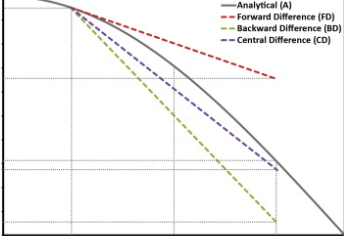
\includegraphics[width=0.45\textwidth]{figures/forward_vs_central_differentiation.png}
%       \caption{Comparison of Forward, Backward, \& Central Differentiation}
%       \label{forward_vs_central}
%       \end{center}
%       \end{figure}
%       \FloatBarrier
% 
% 
% 
% \paragraph{Method Specific Parameters:}
% 
% This section is specific to the method being used. In the above example it is specific to the $OPT++$ library. An additional example has been given below however if curious the reader is advised to see the default optimization methods located in:
% 
% \bigskip
% 
% \begin{lstlisting}
% $./data/cathode/optimization/optimization_methods_cathode/
% \end{lstlisting}
% or 
% \begin{lstlisting}
% $./data/mea/optimisation/optimization_methods_mea/
% \end{lstlisting}
% 
% \bigskip
% 
% In the following short example we are using a method from the SCOLIB library, the \texttt{coliny\_pattern\_search} algorithm. In this case we would change the \texttt{Optimization method = coliny\_pattern\_search} as appose to \texttt{optpp\_q\_newton} (\textit{line 17}).
% 
% We then would then replace (\textit{line 33 - 41}) in the above \texttt{opt\_app\_optimization} file  with the new method specific section.
% 
% \begin{lstlisting}
%      ######### Method Specific Parameters #########
%      #########	      SCOLIB (COLINY) 	   #########
%      #########----------------------------#########
% 	subsection coliny_pattern_search
% 	    set Initial Delta = 2		          # (default) 1
% 	    set Threshold Delta = 0.0001			# (default) 0.0001
% 	end
% \end{lstlisting}
% 
% 
% 
% \paragraph{Design Variables Section:}
% 
% The \texttt{Design Variables} Section is similar to the \texttt{opt\_app\_parametric} file except for two additional subsections.
% 
% \begin{enumerate}
%  \item 
% Scales
% 
% \item
% Step size
% \end{enumerate}
% 
% 
% \paragraph{Scales:} 
% 
% The scales section has two specifications 
% 
% \begin{enumerate}
%  \item 
% \texttt{scale\_method}
% 
% The \texttt{scale\_method} specifies whether you are going to specify no scale (\texttt{none}), \texttt{auto} scaling, \texttt{log}, or a \texttt{value}. In general it is good practice to specify a scale \texttt{value} as it allows the user to have a definite reference point, when using \texttt{auto} if there is a change in magnitude it will go unnoticed by the user in the final output solution. 
% 
% \item
% \texttt{scale} value
% 
% The scale value is the magnitude of the variable. For example if the variable is temperature we know that the scale is 100 as temperature is given in Kelvin (353 - 368 [K]). If its Nafion loading the scale is 0.1 as Nafion loading is a percentage (20 - 50 \%).
% \end{enumerate}
% 
% 
% 
% \paragraph{Step Size:}
% 
% The step size refers to the  $\bigtriangleup x $ in equations \ref{eq:Forward} \& \ref{eq:Central}. Greater the step size the less computations that will be required, however this also means the greatest error as the error is proportional to $(\bigtriangleup x)^2$. Therefore there is a fine trade off between computational time and error.
% 
% 
% 
% \paragraph{Responses Section:}
% 
% The Responses section has changes slightly compared to the \texttt{opt\_app\_parametric} file as we are now considering constrained optimization. If the above example was unconstrained optimization there would be no difference between the \texttt{opt\_app\_parametric} and \texttt{opt\_app\_optimization} responses section.
% 
% There are two types of constraints:
% 
% \begin{enumerate}
%  \item 
% Linear (Equality) Constraints (\textit{line 83})
% 
% \item
% Non-Linear Constraints (\textit{line 84})
% \end{enumerate}
% 
% In the above case we have three non-linear constrains and one linear constraint. 
% 
% 
% 
% \paragraph{Non-Linear Constraints:} 
% 
% Like the \texttt{Design Variable} section each nonlinear constraint requires a upper and lower bound (\textit{line 97 - 108}). If no finite upper or lower bound is to be specified $1e^{30}$ or $1e^{-30}$ can be specified.
% 
% 
% \paragraph{Linear (Equality) Constraints:} Unlike Non-Linear Constraints, Equality constraints only require the response variable to equal a value (\textit{line 112}). 
% 
% 
% 
% 
% 
% %-----------------------------------------------------------------------------------------------------
% %---------------------				Running FCST
% %---------------------			Multi-Objective Optimization
% %-----------------------------------------------------------------------------------------------------
% \section{Multi-Objective Optimization using OpenFCST} \label{sec:multi_objective_optimization}
% 
% To achieve multi-objective optimization we must first change three parameters.
% 
% \begin{enumerate}
%  \item 
% \texttt{Optimization strategy} (\textit{line 16})
% 
% \item
% \texttt{num\_design\_variables} (\textit{line 84})
% 
% \item
% \texttt{num\_objectives} (\textit{line 82})
% 
% \end{enumerate}
% 
% 
% 
% \paragraph{Optimization strategy}
% 
% When carrying out multi-objective optimization we can no longer optimize for just one objective function this is especially the case when an improvement of one objective comes at the expense of another (\textit{Performance \& Cost}). In order account for the additional objective function we incorporate weighting factors which specifies the importance of one objective over the other. The weights are referred to a \textbf{Pareto Weights} or \textbf{Pareto Set}.
% 
% In OpenFCST the default Pareto set is for two design variables. Figure \ref{pareto_set} below shows the  multi-objective weights for two design variables.
% 
% 
% 
% \FloatBarrier
% \begin{figure}[htbp]
% \begin{center}
% 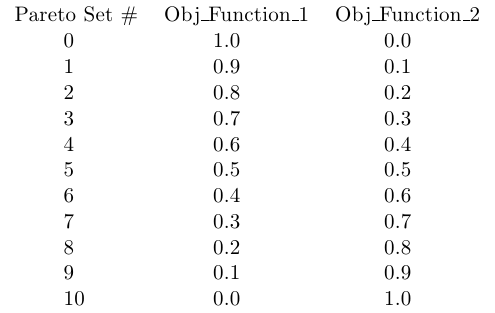
\includegraphics[width=0.4\textwidth]{figures/pareto_set.png}
% \caption{Pareto Set for 2 Design Variables}
% \label{pareto_set}
% \end{center}
% \end{figure}
% \FloatBarrier
% 
% 
% % \begin{center}
% %  
% % 
% % \begin{tabular}{lll}
% % Pareto Set \#	&Obj\_Function\_1 & Obj\_Function\_2 \\
% % 0	&	 1.0 	&	 0.0 	\\
% % 1	&	 0.9 	&	 0.1 	\\
% % 2	&	 0.8 	&	 0.2 	\\
% % 3	&	 0.7 	&	 0.3 	\\
% % 4	&	 0.6 	&	 0.4	\\
% % 5	&	 0.5 	&	 0.5 	\\
% % 6	&	 0.4 	&	 0.6 	\\
% % 7	&	 0.3 	&	 0.7 	\\
% % 8	&	 0.2 	&	 0.8 	\\
% % 9	&	 0.1 	&	 0.9 	\\
% % 10	&	 0.0 	&	 1.0 	\\
% % \end{tabular} 
% % 
% % \end{center}
% 
% 
% 
% \paragraph{num\_design\_variables \& num\_objectives:}
% 
% Once the \texttt{Optimization strategy} has been set to \texttt{pareto\_set} we then change both the num\_design\_variables \& num\_objectives to 2 or whatever number of design variables are specified.
% At present OpenFCST like most multi-objective engineering problems, considers only two design variables however this can be easily modified by changing the default Pareto set found in \texttt{dakota\_application.cc}. 
% 
% \section{DAKOTA Methods} \label{dakota_methods}
% 
% The following list is all of the current DAKOTA Methods available as of \textbf{1-MAY-2013}. The methods are known to work with OpenFCST and can be utilized. For detailed discriptions on the individual methods see DAKOTA manuals.
% 
% \begin{multicols}{3}
% \begin{enumerate}
%     \item 	\textbf{asynch\_pattern\_search}
%     \item       bayes\_calibration
%     \item       centered\_parameter\_study
%     \item       \textbf{coliny\_cobyla}
%     \item       \textbf{coliny\_direct}
%     \item       \textbf{coliny\_ea}
%     \item       \textbf{coliny\_pattern\_search}
%     \item       \textbf{coliny\_solis\_wets}
%     \item       \textbf{conmin\_frcg}
%     \item       \textbf{conmin\_mfd}
%     \item       dace
%     \item       dl\_solver
%     \item       dot
%     \item       dot\_bfgs
%     \item       dot\_frcg
%     \item       dot\_mmfd
%     \item       dot\_slp
%     \item       dot\_sqp
%     \item       \textbf{efficient\_global}
%     \item       fsu\_cvt
%     \item       fsu\_quasi\_mc
%     \item       global\_evidence
%     \item       global\_interval\_est
%     \item       global\_reliability
%     \item       importance\_sampling
%     \item       list\_parameter\_study
%     \item       local\_evidence
%     \item       local\_interval\_est
%     \item       local\_reliability
%     \item       \textbf{moga}
%     \item       \textbf{multidim\_parameter\_study}
%     \item       \textbf{ncsu\_direct}
%     \item       \textbf{nl2sol}
%     \item       nlpql\_sqp
%     \item       nlssol\_sqp
%     \item       nonlinear\_cg
%     \item       npsol\_sqp
%     \item       optpp\_cg
%     \item       \textbf{optpp\_fd\_newton}
%     \item       \textbf{optpp\_g\_newton}
%     \item       optpp\_newton			% Needs the Hessian Matrix
%     \item       \textbf{optpp\_pds}
%     \item       \textbf{optpp\_q\_newton}
%     \item       polynomial\_chaos
%     \item       \textbf{psuade\_moat}
%     \item       richardson\_extrap
%     \item       sampling
%     \item       \textbf{soga}
%     \item       stanford
%     \item       stoch\_collocation
%     \item       surrogate\_based\_global
%     \item       surrogate\_based\_local
%     \item       vector\_parameter\_study
% \end{enumerate}
% \end{multicols}
% 
% 
% 
% 
% 
% 
% 
% %-----------------------------------------------------------------------------------------------------
% %---------------------			Running OpenFCST
% %---------------------			Optimization Path-line
% %-----------------------------------------------------------------------------------------------------
% \section{Fuel Cell Design \& Optimization Using OpenFCST}
% As we've seen above OpenFCST also has the capabilities to perform optimization studies. Any application that is inherited from \texttt{OptimizationBlockMatrixApplication} has the appropriate interface to be used for optimization studies. Information on how to run optimization can be found in sections \ref{Optimization_using_FCST} \& \ref{sec:multi_objective_optimization}.
% 
% To perform optimization studies, OpenFCST interfaces with the open source libraries DAKOTA developed by Sandia National Laboratory. For more information about the DAKOTA library please \href{http://dakota.sandia.gov/software.html}{click here}. The OpenFCST developers have developed an interface so that DAKOTA and OpenFCST can interact seamlessly. 
% 
% \subsection{OpenFCST classes that interact with DAKOTA (Developers Only)}
% Interaction between OpenFCST and DAKOTA is achieved by using \texttt{simulation\_builder} which will call the \texttt{run\_optimization()} function.
% 
% When OpenFCST is run as seen in figure \ref{analysis_schematic} the OpenFCST code is called on once in order to run a specific data point. However in parametric or optimization studies we require multiple points to be evaluated. This requires the use of the DAKOTA libraries in order to change the variables after each iteration. The two main files used to interface with DAKOTA are:
% 
% 
% \begin{enumerate}
%  \item 
% \texttt{dakota\_direct\_interface}
% 
% \item
% \texttt{dakota\_application}
% 
% \end{enumerate}
% 
% Once the initial stages of the code have been carried out by \texttt{simulator\_builder}, \texttt{simulator\_selector}, and \texttt{dakota\_application}, declaring and initialing all the variables from the \texttt{main\_app\_}, \texttt{data\_app\_}, \& \texttt{opt\_app\_} files. The \texttt{main.cc} file then proceeds to the \texttt{run()} function in \texttt{simulator\_builder.cc} (see below) in order to run the simulation.
% 
% In the \texttt{run()} function we can see in line 10 where the code checks to see if its running an analysis or parametric/optimization study, as explained in \ref{main_application_file}. During parametric/optimization studies the code will enter line 12 and proceed to the \texttt{run\_optimization()} function in \texttt{simulator\_builder.cc}. 
% 
% 
% \begin{lstlisting}
% template<int dim>
% void SimulatorBuilder<dim>::run()
% {
% 	timer.restart();
%     
% 	if (run_tests) run_test();
% 	else
% 	{
% 		if (dakota_use || dakota_direct)
% 		{
% 			run_optimization();
% 		}
% 		else
% 		{
% 			//-- Select the application you want to run:
% 			app_lin = sim_selector->select_application();
% 			//-- Select the solver you want to run:
% 			newton = sim_selector->select_solver(app_lin.get());
% 			//-- Select the solving method you want to run, e.g. adaptive refinement:
% 			solver = sim_selector->select_solver_method(app_lin.get(), newton.get());
% 			// Here we have collected all information:
% 			deallog << "Run program using input file: " << simulator_parameter_file_name << std::endl;
% 			deallog.pop();
% 			solver->solve(simulator_parameter_file_name, param);
% 			timer.stop();
% 		}
% 	}
% 
% 	timer.stop();
% 	deallog.push("MAIN");
% 	deallog << "The program was executed in: " << timer.wall_time() << " seconds " << std::endl;
% 	deallog << "=============== END ====================" << std::endl;
% 	deallog.pop();
% 	
% }
% \end{lstlisting}
% 
% \bigskip
% 
% The main points to note once we enter the \texttt{run\_optimization()} function are:
% 
% \begin{enumerate}
% \item 
% Is DAKOTA running in Parallel or Series? (\textit{line 8})
% 
% As of \textbf{1-MAY-2013} Series is the only option available. This may change in the future.
% 
% \item
% Are we running a Non-Linear Least Squares (NLS) method or standard parametric/optimization routine? (\textit{line 16-25})
% 
% \end{enumerate}
% 
% \paragraph{Note:} 
% 
% These are questions that are answered in the \texttt{opt\_app\_} file explained earlier in section \ref{Optimization_using_FCST}.
% 
% 
% \bigskip
% 
% Once these have been specified the code will execute the \texttt{run()} function (\textit{line 28}), which begins the iterative loop until the parametric study has been complete or the stopping criteria have been met in optimization.An illistration of this can be see in figure \ref{dakota_optimization_interface} taken from Peter Dobson's 2012 paper.
% 
% 
% \begin{lstlisting}
% void SimulatorBuilder<dim>::run_optimization()
% {
% 	deallog.pop();
% 	if (dakota_direct)
% 	{
% 		// NOTE: Must declare these in order for parameter handler to not complain when reading the parameter file specified.
% 		//        Not exclusively required for dakota application to run.
% 		Dakota::ParallelLibrary parallel_lib;
% 		shared_ptr<Dakota::ProblemDescDB> problem_db(new Dakota::ProblemDescDB (parallel_lib));
% 		SIM::DakotaApplication optimization(problem_db, optimization_parameter_file_name);
% 		optimization.declare_parameters(param);
% 		optimization.manage_inputs(param);
% 
% 		Dakota::DirectApplicInterface* optimization_interface;
% 		
% 		if (optimization.use_NLS())
% 		{
% 			deallog<<"Entering DakotaLeastSquaresInterface"<<std::endl;
% 			optimization_interface = new SIM::DakotaLeastSquaresInterface<dim> (optimization, problem_db, param, sim_selector, simulator_parameter_file_name);
% 		}
% 		else
% 		{
% 			deallog<<"Entering DakotaDirectInterface"<<std::endl;
% 			optimization_interface = new SIM::DakotaDirectInterface<dim > (optimization, problem_db, param, sim_selector, simulator_parameter_file_name);
% 		}
% 		
% 		optimization.assign_interface(optimization_interface);
% 		optimization.run();
% 		
% 		deallog << "Optimization completed" << std::endl;
% .
% .
% .
% \end{lstlisting}
% 
% 
% If running a standard parametric/optimization routine, the following \texttt{dakota\_direct\_interface} function will be used.
% 
% \begin{lstlisting}
% template <int dim>
% int DakotaDirectInterface<dim>::derived_map_ac(const Dakota::String& ac_name)
% \end{lstlisting}
% 
% If running a Non-Linear Least Squares (NLS) method, the following \texttt{dakota\_direct\_interface} function will be used.
% 
% \begin{lstlisting}
% template <int dim>
% int DakotaLeastSquaresInterface<dim>::derived_map_ac(const Dakota::String& ac_name)
% \end{lstlisting}
% 
% 
% \FloatBarrier
% \begin{figure}[htbp]
% \begin{center}
% 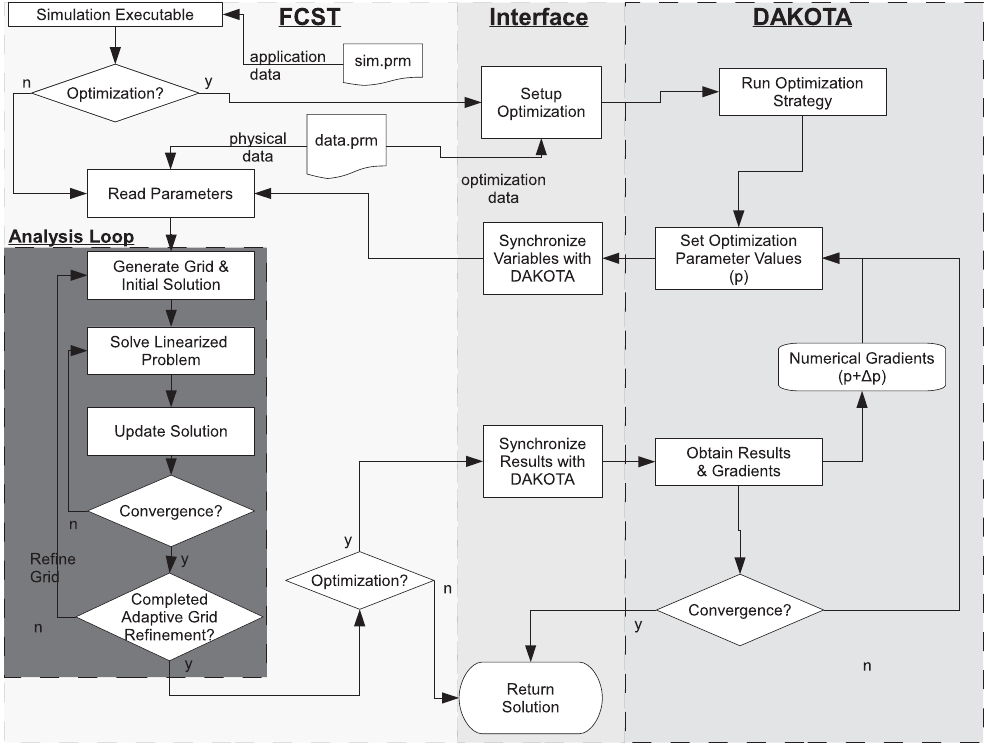
\includegraphics[width=1\textwidth]{figures/fcst_dakota_interface_Dobson.png}
% \caption{Schematic of Fuel Cell Analysis Code and DAKOTA Optimization Interface (Dobson, 2012)}
% \label{dakota_optimization_interface}
% \end{center}
% \end{figure}
% \FloatBarrier

%%===============================================================
%%===============================================================